\section{The \trace Environment}
\label{sec:design}

The taxonomy defines what constitutes a task; the environment instantiates that
definition as a deterministic generator--renderer--verifier pipeline. For each
sampled task, \trace constructs a semantic state, executes the corresponding
task program, renders the image and prompt, and binds the resulting answer and
verifier state to an exact scorer. This design keeps generation, supervision,
and replay grounded in the same underlying state.

\subsection{Executable instance generation}

Each generated instance is represented as
\begin{equation}
  \mathcal{D}_i =
  \bigl(I_i, p_i, y_i, c_i, \tau_i\bigr),
  \label{eq:instance-contract}
\end{equation}
where $I_i$ is the rendered image, $p_i$ is the prompt, $y_i$ is the typed
answer, $c_i$ is the instance-bound scorer, and $\tau_i$ is the corresponding
instance trace. The trace records the semantic state, sampled query, task
execution, rendering decisions, and verifier state, making each instance
replayable and supporting failure analysis.

Let $s$ denote a scene grammar, $t$ a task, $q$ an internal query, $z$ an
instance seed, and $\theta$ the sampled generation parameters. Instance
construction proceeds as
\begin{align}
  x &= G_s(z, \theta_s), &
  (y,v) &= P_t(x;q), \label{eq:semantic-execution}\\
  I &= R_s(x;z,\theta_r), &
  p &= H_{s,t}(x,q;z,\theta_p), \label{eq:render-prompt}\\
  c &= \operatorname{bind}\!\left(\mathcal{C}_t;y,v\right), &
  \tau &= \Gamma(s,t,q,z,\theta,x,v).
  \label{eq:projection-contract}
\end{align}
The scene generator $G_s$ first constructs semantic state $x$. The task
program $P_t$ then executes over that state and returns both the typed answer
$y$ and verifier state $v$. The renderer $R_s$ and prompt function $H_{s,t}$
independently realize the image and question from the same semantic state.
Finally, the task-level reward contract $\mathcal{C}_t$ is bound to the
expected answer and verifier state to produce the instance scorer $c$, while
$\Gamma$ records the complete trace.

Semantic, prompt, and rendering choices are governed by independent seeded
streams. The resulting instance can therefore be reconstructed from its
recorded state without coupling superficial prompt or rendering variation to
the task computation.

\trace supports four answer interfaces: integers, canonical numeric values,
strings, and option letters. Each reward contract specifies the corresponding
type-aware normalization and comparison rule, which the bound scorer applies
to the submitted answer.

Figure~\ref{fig:reachable-pipeline} illustrates the full pipeline for a
cell-board task. A four-neighbor flood fill from the marked start cell produces
the set of reachable passable cells, and the cardinality of that set gives
$y=4$. Passable cells outside the connected region remain visual distractors
but do not enter the task computation.

\begin{figure}[t]
  \centering
  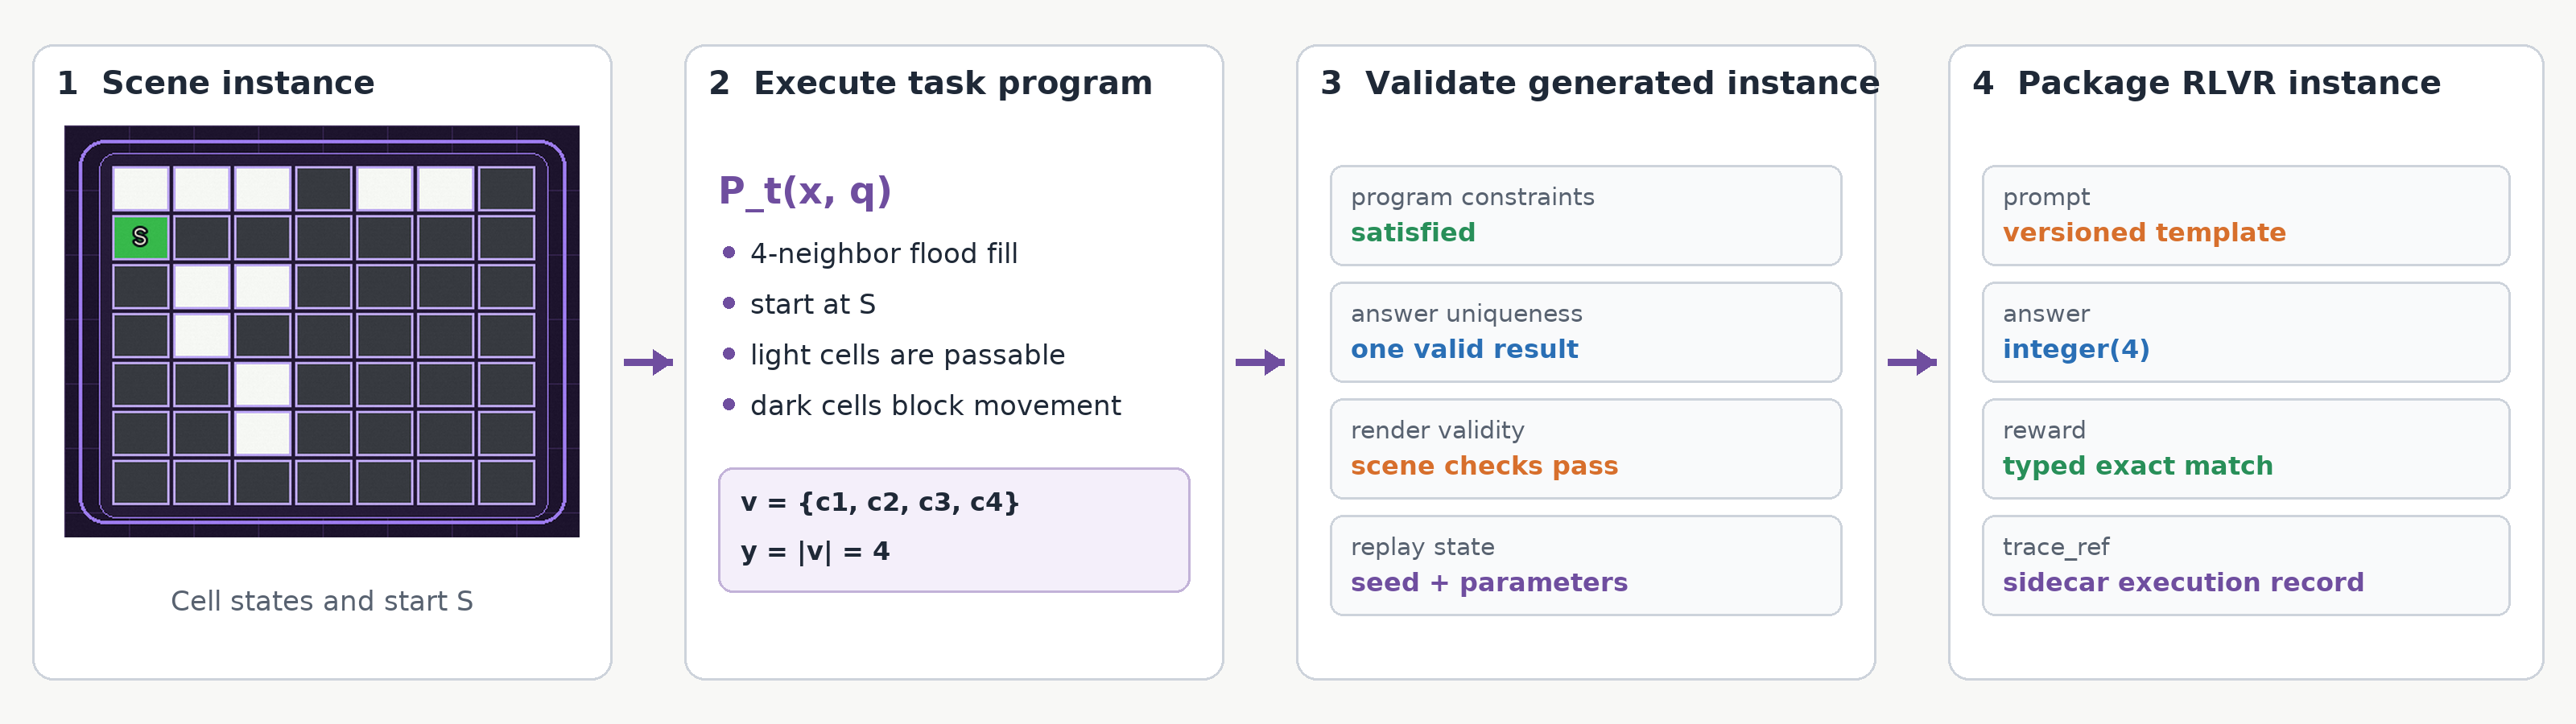
\includegraphics[width=\textwidth]{figures/reachable_region_pipeline.png}
  \caption{End-to-end construction of a \trace instance. Four-neighbor
  reachability is computed over the semantic cell board, and the resulting
  state determines the typed answer, rendered image, prompt, scorer, and
  replayable instance trace.}
  \label{fig:reachable-pipeline}
\end{figure}

\subsection{Environment composition}

\trace comprises 1,000 tasks defined over 277 scene grammars spanning 11
visual domains. The domains organize related visual structures, rendering
conventions, and object vocabularies for reporting and balancing; they are not
themselves reasoning categories or sampling units.
Figure~\ref{fig:environment-composition} summarizes the distribution of tasks,
scene grammars, and answer interfaces across domains.
Figure~\ref{fig:domain-montage} provides representative renderings, and
Appendix~\ref{app:task-atlas} presents a domain-stratified task atlas.

\begin{figure}[t]
  \centering
  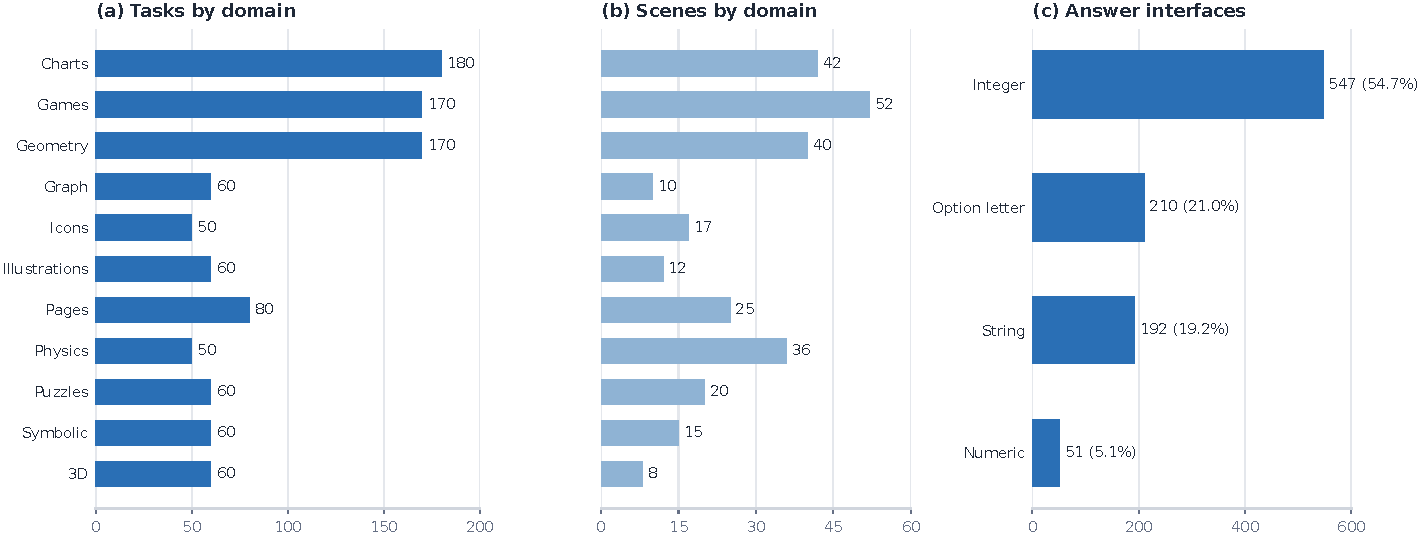
\includegraphics[width=\textwidth]{figures/environment_statistics.pdf}
  \caption{Composition of \trace across 11 visual domains. The panels report
  the number of task programs and scene grammars in each domain, together with
  the overall distribution of answer interfaces.}
  \label{fig:environment-composition}
\end{figure}

The 277 scene grammars support a median of three tasks each
(mean 3.61, range 1--26), indicating that visual construction is reused across
multiple reasoning objectives rather than duplicated for each task. The task
inventory includes integer, canonical numeric, string, and option-letter
outputs; 790 tasks use open-form integer, numeric, or string answers.

Of the 1,000 tasks, 317 expose more than one internal query, producing 1,475
query variants in total. Because task selection precedes query selection,
adding bounded query variants does not increase the sampling probability of the
underlying task. The sampling distribution therefore reflects the authored task
programs rather than the number of prompt-level variants available to each one.

Visual diversity alone does not establish diversity of computation. We
therefore project the task inventory onto 13 compositional operation families,
whose distribution across domains is shown in
Figure~\ref{fig:operation-coverage}. These families are an analytical view of
the task programs rather than an additional taxonomy level. Assignments are
multi-label because a composed program may require several operations; every
task belongs to at least one family, and \emph{direct retrieval} is assigned
only when no other operation materially determines the answer.
Appendix~\ref{app:operation-families} defines the complete set of families.

\begin{figure}[t]
  \centering
  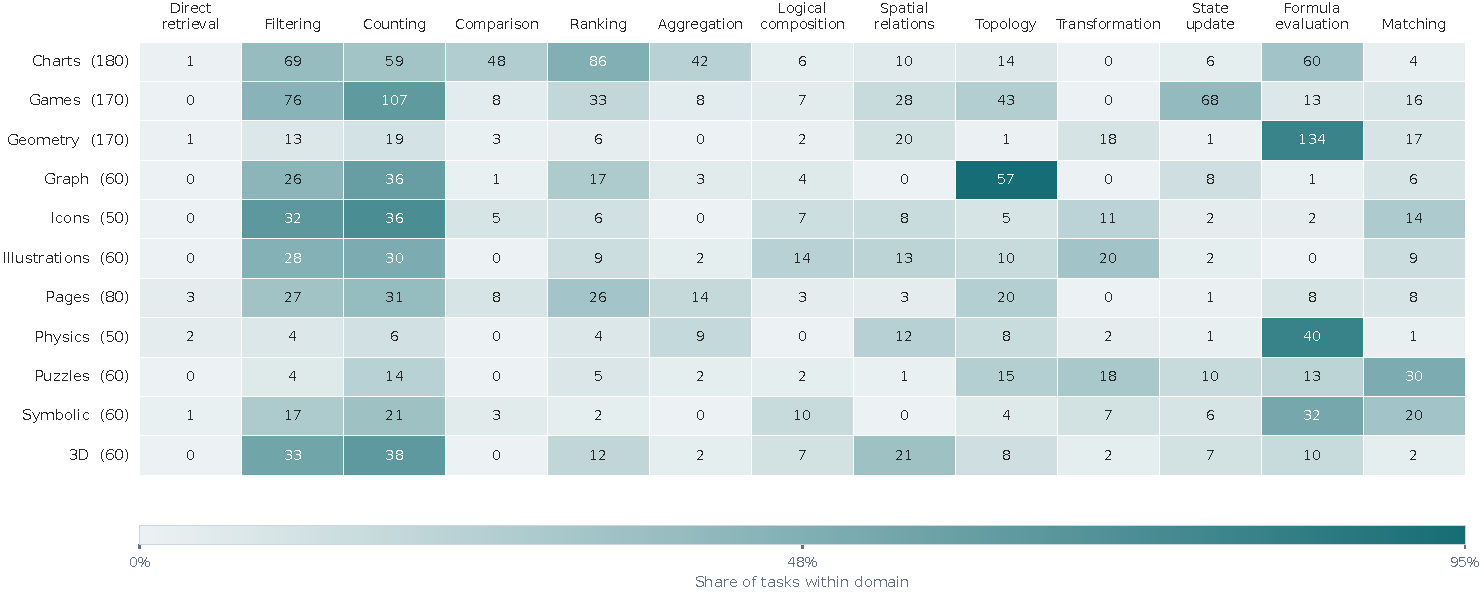
\includegraphics[width=\textwidth]{figures/domain_operation_matrix.pdf}
  \caption{Distribution of task-program operations across visual domains.
  Cell labels report the number of tasks assigned to each operation family,
  while color indicates the corresponding within-domain share. Assignments are
  exhaustive and multi-label.}
  \label{fig:operation-coverage}
\end{figure}

\subsection{Controlled visual realization}

Instance variation occurs at two distinct levels. Semantic controls alter the
state on which the task program operates, including dimensions, cardinalities,
values, thresholds, sequence lengths, and candidate sets. Prompt templates draw
their dynamic labels and values from that same state, ensuring that the
question and answer remain synchronized with task execution. All sampled
choices are retained in the instance trace.

Once semantic execution fixes the state, query, and answer, scene-compatible
realization controls vary how that state is presented. These controls include
placement, panel arrangement, camera, palette, typography, materials,
non-answer context, and bounded raster effects. A realization control is
admitted only when it preserves the relations queried by the task program and
therefore leaves the typed answer unchanged. Appendix~\ref{app:generation}
formalizes these variation layers and their required invariants.

For information-rich scenes, \trace may additionally introduce curated
context outside answer-bearing regions. Such context is constrained by
scene-specific fit, collision, and contrast checks so that visual complexity
can increase without modifying the underlying task state.

\begin{figure}[t]
  \centering
  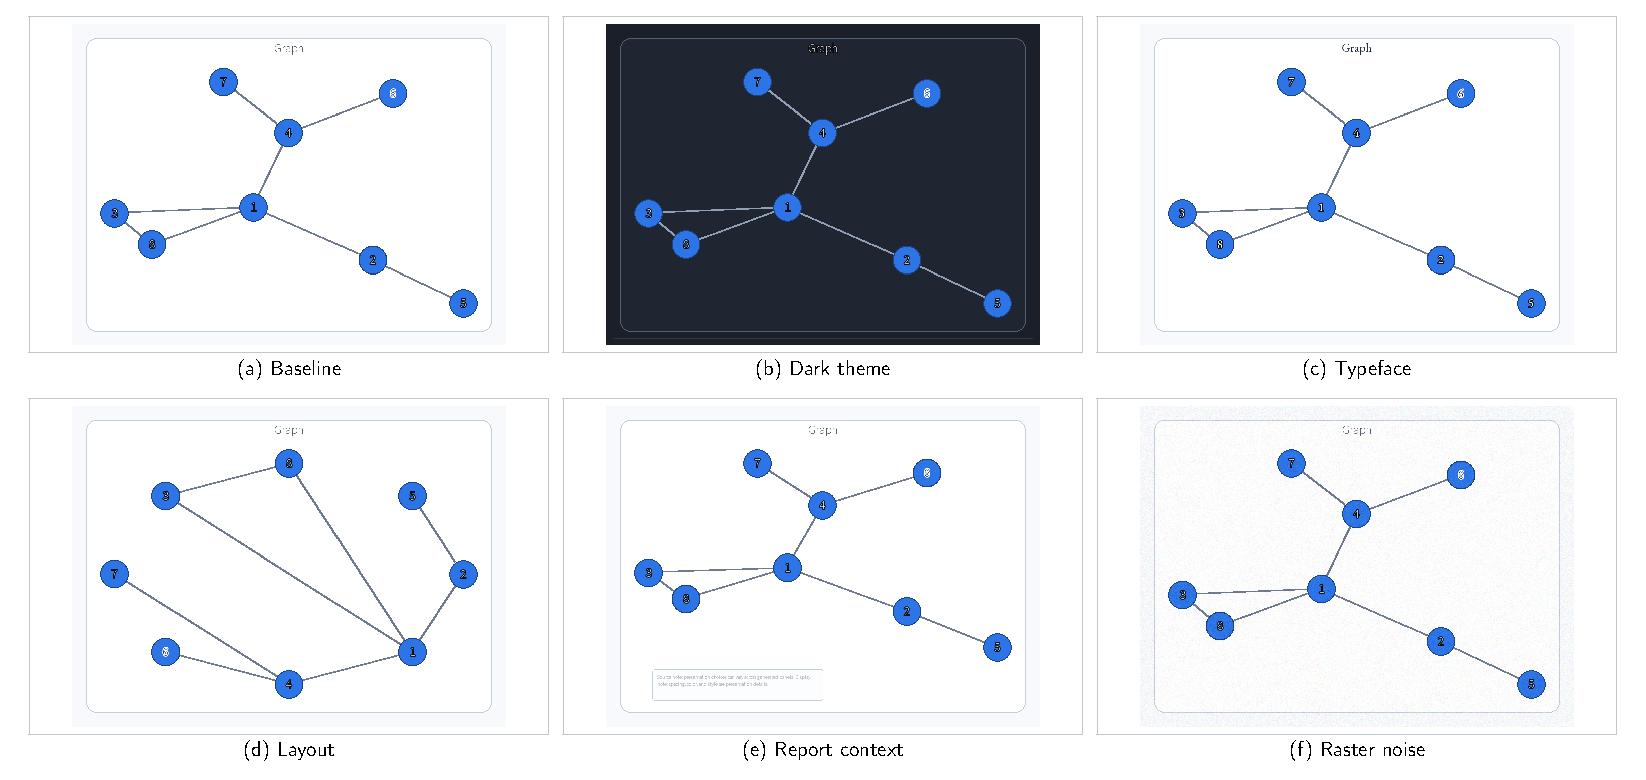
\includegraphics[width=0.72\textwidth]{figures/rendering_variation_examples.pdf}
  \caption{Answer-preserving realizations of a fixed semantic graph. Theme,
  typeface, layout, non-answer context, and raster treatment vary while the
  prompt, topology, query, and typed answer remain unchanged.}
  \label{fig:rendering-variation}
\end{figure}

\subsection{Instance validation}

An instance is retained only if task execution produces a unique typed answer,
the prompt and rendered image remain consistent with the semantic state, and
deterministic replay reconstructs the same instance. Scene-specific rendering
checks additionally test visibility, contrast, fit, and collisions.

These structural checks cannot guarantee that every generated question is
semantically clear or that every valid rendering is equally legible. We
therefore also inspect samples from every task for semantic clarity,
prompt--image consistency, and visual legibility, complementing automatic
validation with direct review of the rendered instances.
